\documentclass[11pt]{article}
\usepackage[margin=1in]{geometry}
\usepackage{amsmath,amssymb}
\usepackage{booktabs}
\usepackage{graphicx}
\usepackage{hyperref}
\usepackage{xcolor}
\usepackage{titlesec}
\usepackage{enumitem}
\hypersetup{colorlinks=true,linkcolor=black,citecolor=blue,urlcolor=blue}
\titleformat{\section}{\large\bfseries}{\thesection}{0.6em}{}
\titleformat{\subsection}{\normalsize\bfseries}{\thesubsection}{0.6em}{}

\title{\textbf{Open-Box: Punching Above the VRAM Weight Class}\\[0.3em]
\large A reproducible research program for running larger effective models on small GPUs}
\author{Mark Bartlett\\ \small InsiderLLM \quad \texttt{mark@insiderllm.com}\\ \small \url{https://github.com/msb-msb/openbox-llm}}
\date{July 2026}

\begin{document}
\maketitle

\begin{abstract}
\noindent
Most ``open'' language models publish weights but not the means to rebuild them, and most
efficiency research targets datacenter-scale hardware. We describe \emph{Open-Box}, a research
program with a single organizing thesis: \emph{decouple a model's effective capability from what
must reside in GPU VRAM}. Under this thesis we identify complementary bets---sparse attention,
trainable memory layers, explicit hot/cold weight offload, and knowledge injection as an
alternative to retrieval---each trading scarce VRAM for more abundant compute, host memory, or
disk. As the program's first validated component, we present a clean-room, reproducible
implementation of Native Sparse Attention (NSA)~\cite{nsa} with custom Triton kernels, gated for
correctness against a reference at every construction step. We validate the kernels across
attention configurations, confirm portability from Ampere (\texttt{sm\_86}) to Hopper
(\texttt{sm\_90}) with all gates green, and report a $+53\%$ end-to-end training throughput
improvement from a query-tiling optimization on the contiguous-range branches. We pair this with
an honest negative result and a diagnosis: the same optimization does not transfer to the
selection branch, and a per-branch profile shows selection is in fact the \emph{dominant} training
cost ($52.6\%$ of a step, driven by its backward pass). A roofline analysis explains why---the
selection branch is latency-bound, not compute-bound. Restructuring the selection backward
block-outer and atomics-free, following concurrent NSA-kernel work~\cite{fsa}, then makes it
$8.4\times$ faster at the 1.5\,B shape and yields a $1.63\times$ end-to-end training-step speedup,
turning the dominant cost into a minor one. We release weights, data, training code,
and kernels under a permissive license. Our contribution is not the invention of NSA (due to
DeepSeek-AI~\cite{nsa}) but its open, reproducible realization, cross-architecture validation, and
honest performance characterization, positioned as the substrate for the broader program.
\end{abstract}

\section{Introduction}
Attention's $O(T^2)$ cost dominates long-context training and inference, and sparse attention has
emerged as the leading remedy. Native Sparse Attention (NSA)~\cite{nsa} is a state-of-the-art
instance: a natively-trainable design combining compression, selection, and sliding-window branches
that matches full-attention quality while cutting FLOPs. Its efficiency, however, lives in
hand-written kernels, and the open implementations of those kernels are typically tuned to one GPU
generation and not validated across others---a gap that matters most to the practitioners least able
to absorb it.

That audience is the one running models on a single consumer or workstation GPU, where the binding
constraint is not compute but \emph{VRAM}: a 24\,GB card caps parameters, KV cache, and activation
memory alike. Datacenter-scale efficiency work rarely targets this regime. The practical goal is to
make a small GPU behave like a larger one.

We present \emph{Open-Box}, a research program organized around one thesis---\emph{decouple a
model's effective capability from what must reside in GPU VRAM}---and its first validated component.
Each part of the program spends an abundant resource (compute, host RAM, disk, an explicit index) to
relieve the scarce one (VRAM); we state the full set of bets, labeled by confidence, in
\S\ref{sec:program}. This paper's concrete contribution is a clean-room, reproducible NSA
implementation whose Triton kernels are gated against a reference at every step and validated from
Ampere (\texttt{sm\_86}) to Hopper (\texttt{sm\_90}). We report a $+53\%$ training-throughput
optimization on the contiguous-range branches, an honest negative result on the selection branch,
and a profile showing selection dominates the training step ($52.6\%$)---a finding independently
corroborated by concurrent NSA-kernel work~\cite{fsa}. Acting on that profile, we rebuild the
selection backward block-outer and atomics-free, making it $8.4\times$ faster and the whole training
step $1.63\times$ faster. We claim no large trained model; our own
throughput measurements (\S\ref{sec:perf}) show why one is a funded, not incidental, undertaking. We
position Open-Box as an open, reproducible \emph{substrate} and program, not a faster kernel than
the specialized implementations~\cite{fsa,nosa} we build on.

\paragraph{Contributions.}
\begin{itemize}[leftmargin=1.2em,itemsep=2pt]
\item A statement of the Open-Box research program and its thesis (\S\ref{sec:program}), each bet
labeled by how proven it currently is.
\item A clean-room, reproducible NSA implementation built as a gated ``rung ladder,''
correctness-checked against a reference at every step (\S\ref{sec:impl}--\ref{sec:validation}).
\item Cross-architecture validation from Ampere to Hopper, all gates green (\S\ref{sec:portability}).
\item Two measured optimizations---a $+53\%$ query-tiling gain on the range branches and an
$8.4\times$ block-outer rebuild of the dominant selection backward ($1.63\times$ end-to-end)---with
a roofline analysis and an honest negative result explaining which fix applies where (\S\ref{sec:perf}).
\item Full release of weights, data, code, and kernels under a permissive license.
\end{itemize}

\section{The Open-Box Program}
\label{sec:program}
The thesis---decouple capability from VRAM---is realized by a small architecture and a set of bets.

\paragraph{Architecture.} A compact reproducible \emph{base} model, a \emph{growable memory store},
and \emph{explicit-selection offload}. The base is small enough to understand and train on modest
hardware. Capacity grows by adding memory entries rather than retraining. Because selection is
explicit (a lookup, not a learned prediction), residency of weights across GPU / host / disk is
tractable to schedule.

\paragraph{The bets.} We label each by current confidence, because a research program stated
honestly is more useful than one stated optimistically:
\begin{itemize}[leftmargin=1.2em,itemsep=2pt]
\item \textbf{Native Sparse Attention (NSA)}~\cite{nsa} --- \emph{validated here.} Reduces
attention's $O(T^2)$ cost via compression, selection, and sliding-window branches. The subject of
this paper.
\item \textbf{Trainable memory layers}~\cite{memlayers} --- \emph{published, our bet to validate at
scale.} Capacity in an addressable store rather than dense parameters; the mechanism by which the
base ``grows'' without retraining.
\item \textbf{Hot/cold offload} --- \emph{the mechanism that makes the small-GPU goal real.} Keep
hot weights in VRAM, cold weights in host RAM or on disk, and swap by need. PowerInfer~\cite{powerinfer}
\emph{predicts} activation with an auxiliary model; explicit top-$k$ memory selection instead makes
``which weights are cold this token'' a lookup rather than a forecast. Concurrent work on
offloadable sparse attention (NOSA~\cite{nosa}) demonstrates the block-wise GPU/CPU swapping this
bet depends on.
\item \textbf{Knowledge injection vs.\ retrieval} --- \emph{most speculative.} Inject a document's
knowledge directly into memory---editable and inspectable---rather than retrieving chunks into
context. We build on Hay's LARQL~\cite{larql}, which decompiles a model into a queryable index and
edits its knowledge without retraining; the open question is whether injected knowledge recalls
\emph{faithfully} at document scale versus a retrieval baseline. In our own prior experience the
tooling (document $\to$ text) is trivial; faithful recall is the hard part.
\end{itemize}
All bets spend abundant resources to relieve VRAM. This paper validates the first and establishes
the substrate the rest depend on.

\section{Background: Native Sparse Attention}
\label{sec:background}
NSA~\cite{nsa} replaces dense attention with three branches whose outputs are gated and summed.
For query $q_t$ at position $t$, with keys/values partitioned into blocks of size $B$,
\begin{equation}
o_t = \sum_{c\,\in\,\{\mathrm{cmp},\,\mathrm{sel},\,\mathrm{win}\}} g_t^{c}\;\mathrm{Attn}\!\left(q_t,\,\tilde{K}_t^{c},\,\tilde{V}_t^{c}\right),
\qquad g_t^{c}\in[0,1],
\end{equation}
where $g_t^{c}$ are learned gates and $(\tilde{K}_t^{c},\tilde{V}_t^{c})$ are the keys/values each
branch attends:

\begin{itemize}[leftmargin=1.2em,itemsep=3pt]
\item \textbf{Compression.} Blocks are pooled into summaries
$\tilde{K}_t^{\mathrm{cmp}}=f_K(K_{\le t})$, giving cheap global coverage over $\lceil t/B\rceil$
entries.
\item \textbf{Selection.} Block importance is scored from the compression branch,
$p_t=\mathrm{softmax}(q_t\tilde{K}_t^{\mathrm{cmp}\top})$, and the top-$k$ blocks are gathered at
full resolution: $\mathcal{I}_t=\mathrm{Topk}(p_t)$, $\tilde{K}_t^{\mathrm{sel}}=K[\mathcal{I}_t]$.
Crucially $\mathcal{I}_t$ is computed under $\mathrm{stopgrad}$---no gradient flows through the block
choice. Preserving this (we call it \emph{trap-1}) is a correctness invariant throughout.
\item \textbf{Sliding window.} The most recent $w$ tokens $\tilde{K}_t^{\mathrm{win}}=K_{t-w:t}$ are
attended densely for local structure.
\end{itemize}

Compression and window both attend a \emph{contiguous causal range}; selection attends a
\emph{scattered, per-query} set of blocks---a distinction that turns out to govern which
optimizations apply (\S\ref{sec:perf}). We use grouped-query attention (GQA) and implement the
kernels in Triton~\cite{triton}.

\section{Implementation}
\label{sec:impl}
We build the implementation as a \emph{rung ladder}: each rung is a self-contained step that must
pass a correctness gate before the next begins, so regressions stay local and every claim is backed
by a green gate.

\begin{enumerate}[leftmargin=1.4em,itemsep=2pt]
\item \textbf{Pure-PyTorch NSA} --- a readable reference implementation of all three branches.
\item \textbf{Selection forward kernel} --- a Triton kernel for the selection branch's
gather-and-attend, using an online softmax to avoid materializing the attention matrix, matched
against the reference.
\item \textbf{Selection backward kernel} --- gradients $dQ, dK, dV$, gated by gradient parity
against autograd through the reference. Softmax statistics are handled explicitly; \emph{trap-1}
keeps block selection non-differentiable.
\item \textbf{Fusion} --- compression and window, which both attend a contiguous causal range
$[\text{lo},\text{hi}]$, are unified into one range-attention kernel; the three branches are
combined via autograd rather than a monolithic fused backward.
\item \textbf{Model integration} --- the fused path is wired into the model behind a flag,
defaulting to the reference path, so kernel-path training is opt-in and verifiable.
\end{enumerate}

\section{Validation}
\label{sec:validation}
\paragraph{Correctness.} Each kernel is gated by \texttt{allclose} against the reference across a
configuration matrix spanning batch size, GQA group ($G\in\{1,2,3,4\}$), head dimension
($D\in\{32,64,128\}$), sequence length, block size, and selection counts exceeding a row's valid
block span. Forward, backward (via gradient parity), and the fused three-branch path all pass in
both \texttt{fp32} and \texttt{bf16}, with maximum errors well inside tolerance (forward
$\max_\text{abs}\approx5.4\times10^{-7}$; backward worst-case $|\Delta g|\approx2.5\times10^{-6}$ in
\texttt{fp32} against a $3\times10^{-3}$ gate).

\paragraph{Model-level parity.} Wired into the full model, the kernel path matches the reference on
both loss and per-parameter gradients, confirming the flag is a true drop-in that does not alter
training dynamics.

\paragraph{Quality.} On a matched-baseline comparison at 152.96\,M parameters
(\texttt{d768/L16}, GQA 12q/4kv) trained on FineWeb-Edu, NSA reaches a held-out validation loss of
$5.44$ versus $5.42$ for full attention---a $+0.53\%$ gap, i.e.\ competitive quality alongside the
memory benefit below. The kernel path tracks the reference step-for-step
(Fig.~\ref{fig:valloss}).

\paragraph{Memory scaling.} At the model level the fused path uses $7.77$\,GB versus $14.05$\,GB for
dense at matched configuration ($-44.7\%$), and remains resident at sequence lengths where dense
runs out of memory (Fig.~\ref{fig:vram}).

\begin{figure}[t]
\centering
\begin{minipage}{0.48\textwidth}\centering
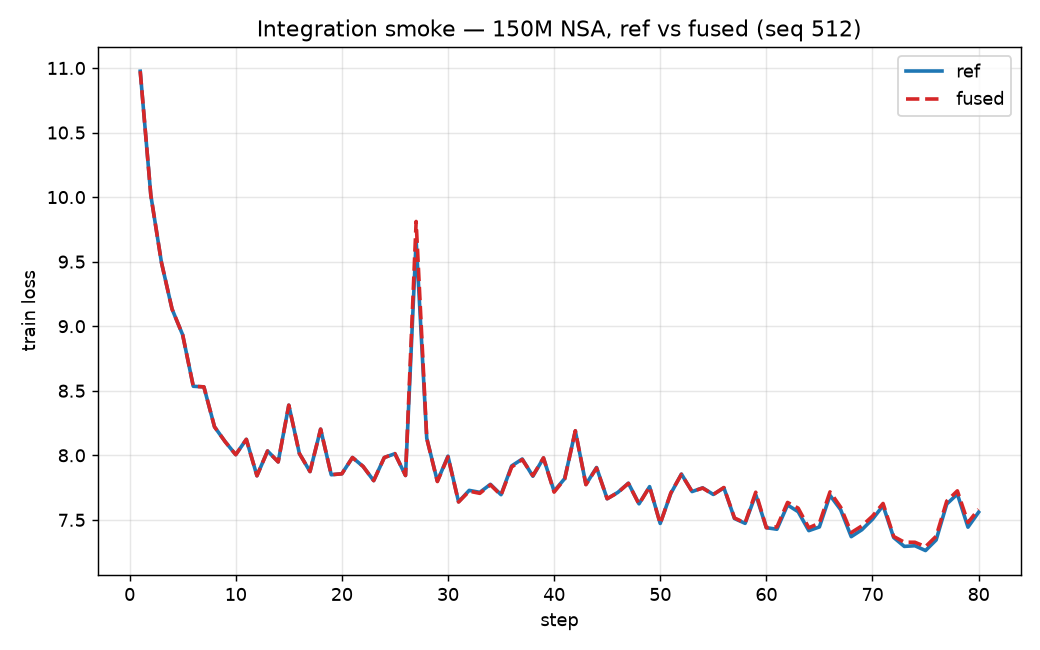
\includegraphics[width=\linewidth]{integration_loss.png}
\caption{Model-level loss parity, 152.96\,M params: the fused kernel path tracks the reference
step-for-step, confirming a true drop-in.}
\label{fig:valloss}
\end{minipage}\hfill
\begin{minipage}{0.48\textwidth}\centering
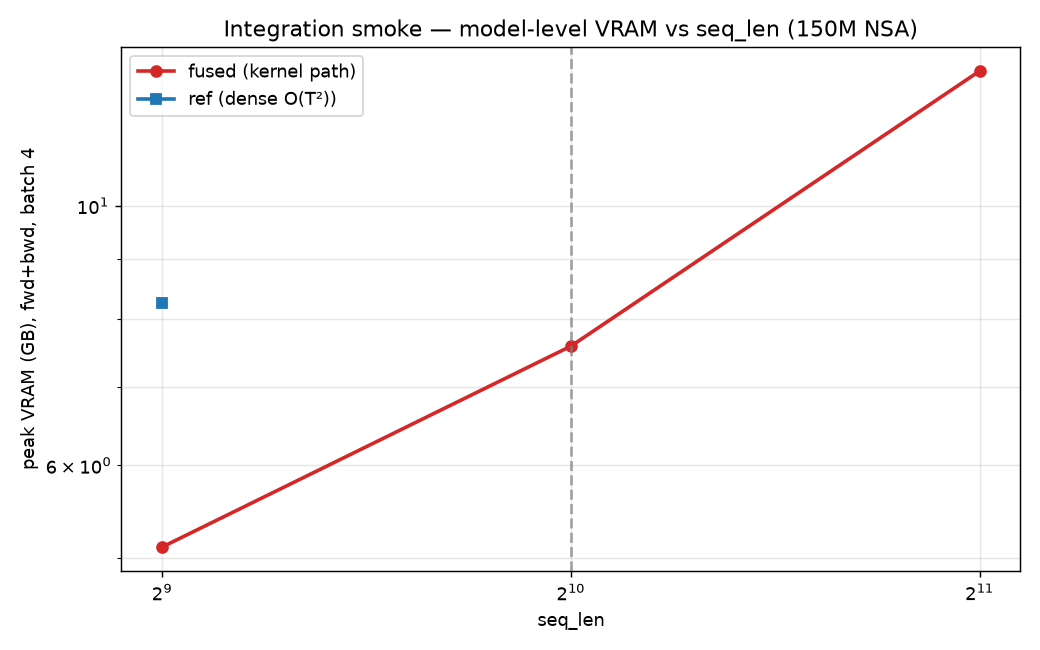
\includegraphics[width=\linewidth]{integration_vram.png}
\caption{Model-level VRAM vs.\ sequence length: fused NSA stays resident where dense OOMs ($-45\%$).}
\label{fig:vram}
\end{minipage}
\end{figure}

\section{Cross-Architecture Portability}
\label{sec:portability}
The kernels were developed and gated on an Ampere RTX~3090 (\texttt{sm\_86}). We re-ran the full
gate suite---forward, backward, fused, and model integration---on a Hopper H100 (\texttt{sm\_90})
without source changes. The Triton autotuner re-tunes per device; no architecture-specific code was
required. All gates passed in both \texttt{fp32} and \texttt{bf16}, establishing portability across
two GPU generations and validating the implementation on the architecture intended for larger runs.

\section{Performance Analysis}
\label{sec:perf}
\paragraph{Query-tiling ($+53\%$ training).} The range-attention kernel (compression and window)
initially padded the GQA group to the hardware matrix-multiply row floor, underusing tensor cores.
By tiling multiple query blocks per program so adjacent queries share a contiguous key range, the
MMA tiles fill with real work. This raised the fused \emph{forward} microbenchmark by $+46\%$ at
sequence length 2048 (the window branch alone improved $4.3$--$4.8\times$; the whole-forward figure
is diluted by the unchanged selection branch), and lifted \emph{end-to-end} training throughput by
$+53\%$ ($5{,}765\to8{,}807$ tokens/s, 198\,M params, RTX~3090), with all correctness gates green
(Fig.~\ref{fig:qtile}). Backward benefits as well as forward, and backward dominates training, so
the end-to-end gain exceeds the forward microbenchmark.

\paragraph{An honest negative: selection does not tile.} Applying the same query-tiling to the
selection branch does not work, and the reason is structural. Unlike the range branches, selection
performs a \emph{per-query} top-$k$ gather, so adjacent queries do not share a key range; stacking
their blocks to fill the MMA merely moves padding from rows to columns while conserving total work.
A roofline measurement confirms the branch is neither compute- nor bandwidth-bound---at a
representative configuration it reaches only a few percent of peak on either axis. It is
\emph{latency/occupancy-bound}: many small programs each chasing a short chain of dependent gather
loads through a masked online softmax. A flash-decode-style split adding parallelism produced no
improvement (within noise), consistent with the kernel already saturating occupancy.

\paragraph{Where the cost actually is.} A per-branch profile of a full training step at 1.5\,B
parameters (Fig.~\ref{fig:breakdown}) shows selection is the \emph{dominant} cost at $52.6\%$ of the
step---almost entirely its backward pass ($45.0\%$ backward vs.\ $7.6\%$ forward). Dense
feed-forward and projections account for $19.3\%$, the range branches $18.6\%$, and everything else
$9.5\%$. Measured model FLOPs utilization is $\sim$32\% against the RTX~3090's honest bf16 peak of
$\sim$35\,TFLOP/s (the card halves throughput under fp32 accumulation, so this peak---not the
nominal 71\,TFLOP/s---is the correct denominator). The optimization that worked addressed the range
branches; the branch that dominates is precisely the one it cannot help. The route forward is not
wider MMA tiles but reducing the selection backward's overhead.

\paragraph{Rebuilding the selection backward ($8.4\times$).} We restructured the selection backward
along the lines of concurrent NSA-kernel work~\cite{fsa}, in dependency order: (i) emit the
log-sum-exp statistic from the forward pass and build a causal, block-to-query inverted index (CSR);
(ii) rewrite $dK/dV$ block-outer---one program owns a KV block, loads it once, and loops the real
queries that selected it, so the matrix-multiply tile fills without GQA padding and the scatter needs
no atomics; (iii) make $dQ$ block-outer as well, fusing $dq=ds\,K$ into the same pass and consuming
the stored statistic in a single softmax pass. Each step preserved \emph{trap-1} (the block index
stays non-differentiable), and a shape gate retains the original kernel for the small configurations
where the restructured path's fixed cost would not amortize. All correctness gates stayed green and
kernel-vs-reference gradient parity held ($\text{fp32}\lesssim10^{-5}$). At the 1.5\,B shape the
selection backward drops from $23.3$ to $3.03$\,ms ($8.4\times$; $87.9\text{k}\to676\text{k}$
tok/s), taking the branch from $45\%$ of the step to $\sim$10\% and yielding a measured $1.63\times$
end-to-end training-step speedup (Fig.~\ref{fig:fsa})---turning the dominant cost into a minor one
and lowering the wall-clock (and dollar) cost of any run by the same factor. This end-to-end figure
is hardware-dependent: on an H100 the same rebuild gives a smaller $1.14\times$ step speedup, because
the H100's much faster dense matmul shrinks selection's share of the step. The branch speedup itself
transfers (the kernel gates pass on \texttt{sm\_90}); its end-to-end impact scales with how large a
fraction the selection backward was to begin with.

\paragraph{Selection forward.} Applying the same block-outer restructuring to the selection
\emph{forward} (a split-K structure emitting per-query softmax partials into CSR-indexed buffers,
combined by log-sum-exp) makes it $1.57\times$ faster in isolation at the 1.5\,B shape
($4.28\to2.40$\,ms; up to $2.4\times$ at larger head dimension). Since the forward is only
$\sim$7.6\% of the step, the incremental end-to-end gain is small ($1.034\times$ over the
backward-only result), bringing the combined kernel speedup to $\sim$1.69$\times$. A stricter shape
gate ($D\ge128$) keeps the original path where the CSR overhead would not amortize.

\begin{figure}[t]
\centering
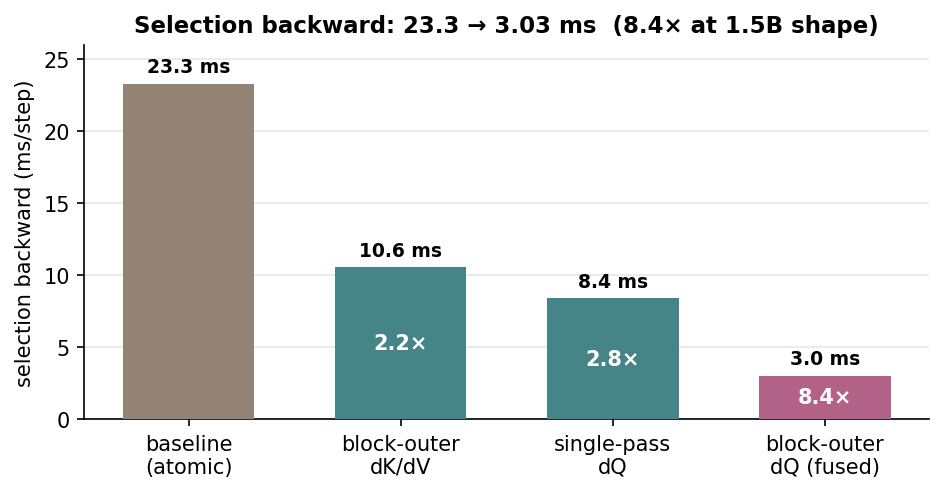
\includegraphics[width=0.62\linewidth]{fsa_progression.png}
\caption{Rebuilding the selection backward in dependency order. At the 1.5\,B shape the branch drops
$23.3\to3.03$\,ms ($8.4\times$), all correctness gates green throughout.}
\label{fig:fsa}
\end{figure}

\begin{figure}[t]
\centering
\begin{minipage}{0.52\textwidth}\centering
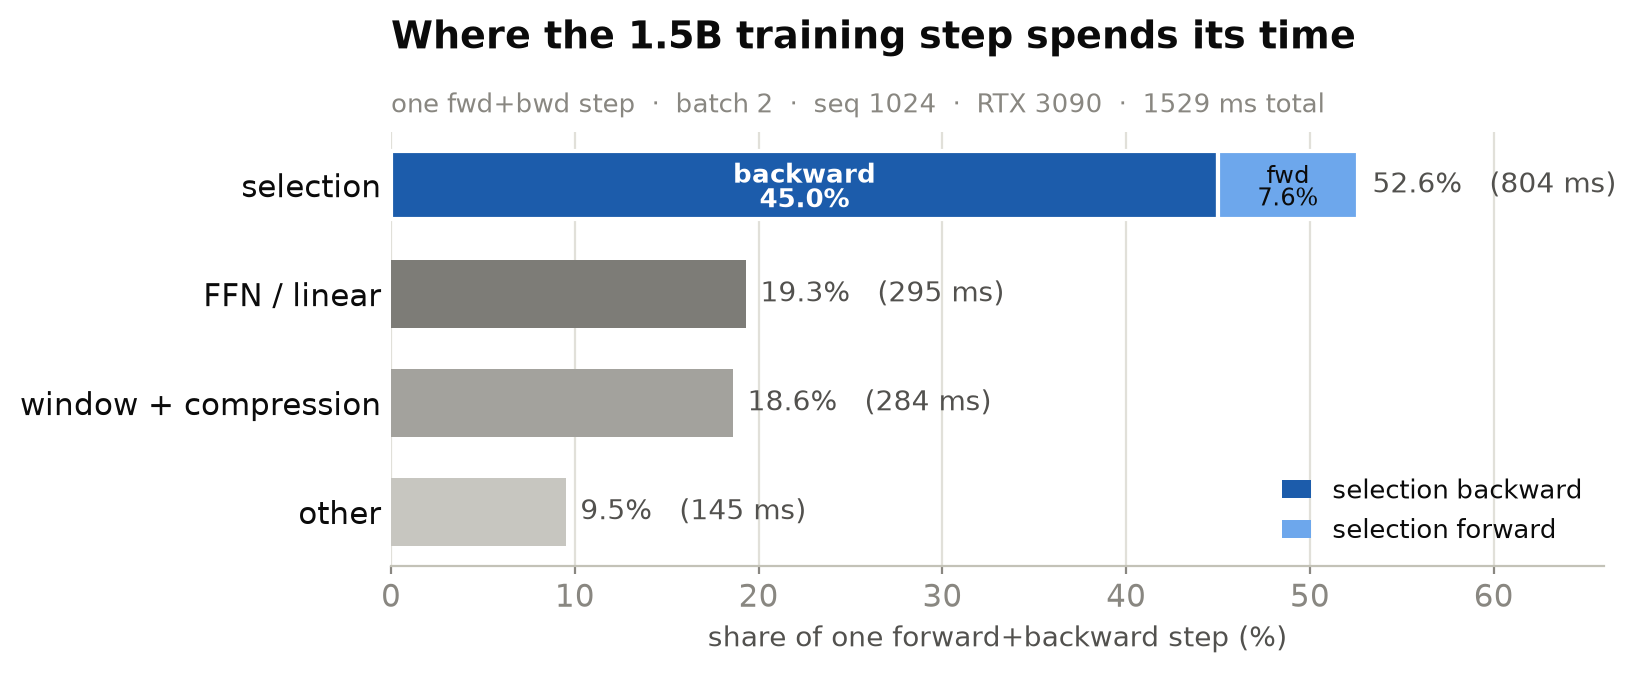
\includegraphics[width=\linewidth]{branch_breakdown.png}
\caption{Per-branch share of a 1.5\,B fwd+bwd training step. Selection dominates ($52.6\%$),
driven by its backward.}
\label{fig:breakdown}
\end{minipage}\hfill
\begin{minipage}{0.44\textwidth}\centering
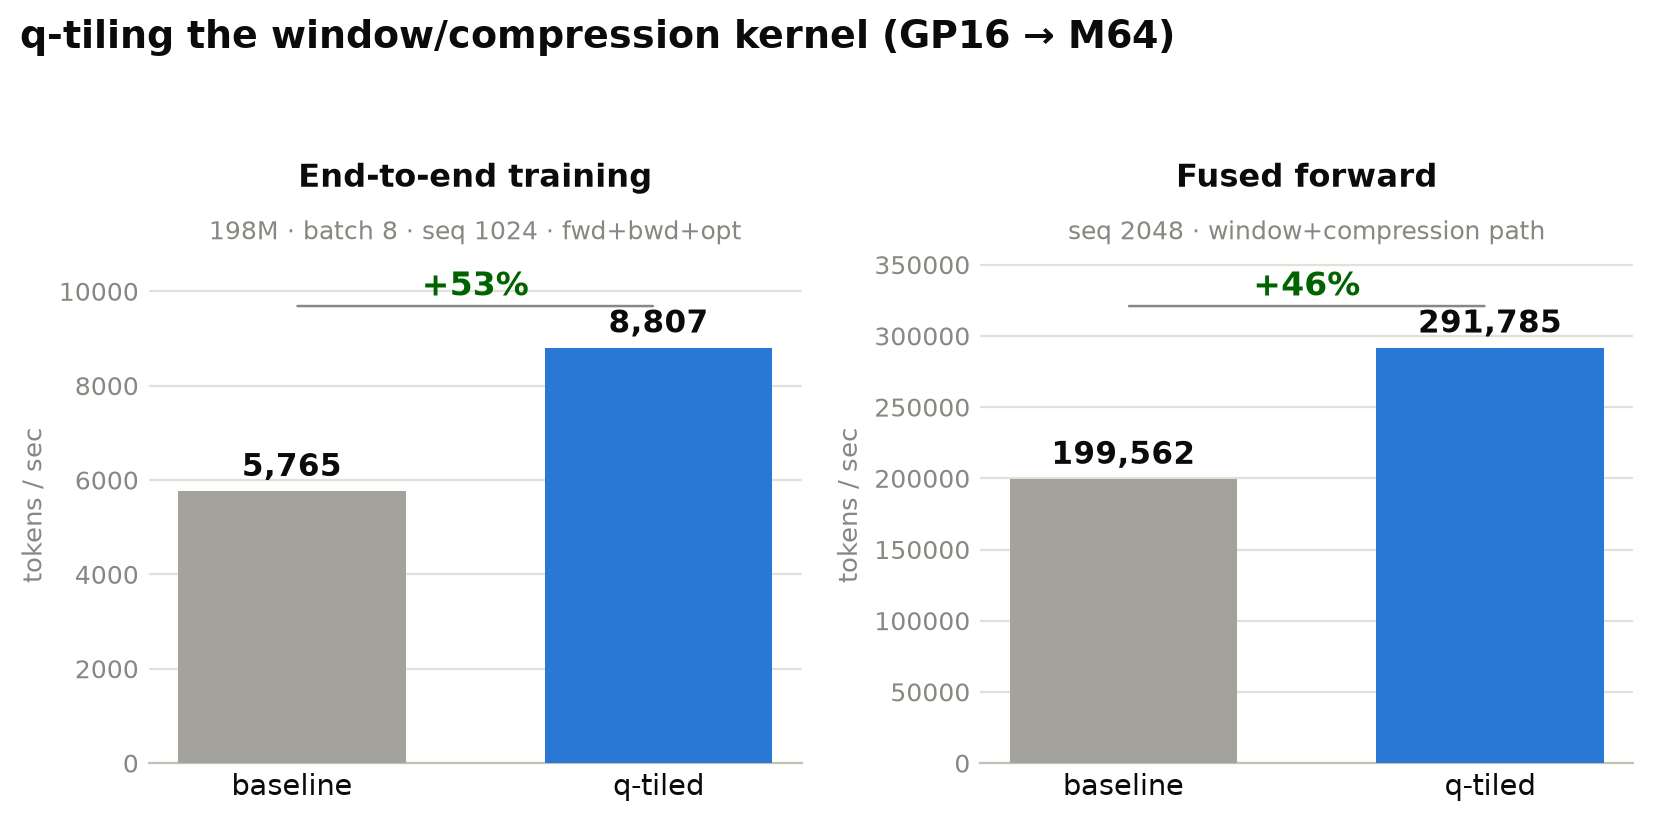
\includegraphics[width=\linewidth]{qtile_speedup.png}
\caption{Query-tiling: end-to-end training $+53\%$ and fused-forward $+46\%$ (seq 2048).}
\label{fig:qtile}
\end{minipage}
\end{figure}

\section{Related Work}
\label{sec:related}
NSA~\cite{nsa} introduced the compression/selection/window design and hardware-aligned Triton
kernels, validated at 27\,B parameters. Our work is an independent, open reproduction at consumer
scale with cross-architecture validation, not a novel mechanism.

Flash Sparse Attention (FSA)~\cite{fsa} is the closest peer: an alternative NSA-kernel implementation
that inverts the vanilla loop order (KV blocks outer, query tokens inner) so a full tile of queries
attends each KV block, eliminating the GQA-group padding that starves tensor cores when groups are
small. It handles the resulting cross-block reduction with a decoupled online-softmax pre-computation
kernel and a separate reduction kernel, avoiding atomics. FSA reports up to $3.5\times$ (avg
$1.6\times$) kernel-latency and up to $1.25\times$ (avg $1.09\times$) end-to-end training speedups.
Two points connect directly to us: FSA's padding diagnosis is the same one our query-tiling addresses
for the range branches; and FSA's own breakdown finds token selection dominates attention cost (up to
$79\%$, avg $65\%$), independently corroborating our $52.6\%$ selection profile. We adopt their
block-outer, atomics-free restructuring for our selection backward (\S\ref{sec:perf}), reaching
$8.4\times$ on that branch at the 1.5\,B shape; we do not claim to match FSA's fully-tuned kernel,
but the same design principles transfer to our open substrate.

NOSA~\cite{nosa} makes NSA-style selection natively offloadable, constraining CPU$\to$GPU KV transfer
via a locality-bounded, block-wise selection so that decoding stays communication-cheap---prior art
for our hot/cold offload bet.

Relative to all three, our contribution is reproducibility and open release, cross-generation
($\texttt{sm\_86}\to\texttt{sm\_90}$) validation, and situating NSA within a broader VRAM-decoupling
program. We do not claim faster kernels than FSA; where speed is the goal, FSA's design is the one to
adopt.

\section{Limitations and Research Program}
We deliberately claim no large trained model. Our throughput measurements show a compute-optimal
1.5\,B run remains a datacenter-budget undertaking on rented hardware even after the $1.63\times$
speedup---the selection-backward rework lowers the cost but does not eliminate the need for funded
compute. What we establish is the \emph{substrate}: correct, portable, and---after the rework of the
dominant branch---reasonably efficient NSA kernels, with a performance envelope characterized
honestly and its worst cost identified and then removed.

\paragraph{Roadmap.} The program proceeds by \emph{component}, not by model size, each step gated by
the last:
\begin{enumerate}[leftmargin=1.4em,itemsep=2pt]
\item \textbf{Distillation from a larger open teacher} --- with the base trained, distill from an
open 27--35\,B teacher (logit/KL) to lift a small-token-budget 1.5\,B student to a usable capability
level; the substrate the bets below are tested on.
\item \textbf{Trainable memory layers}~\cite{memlayers} at the current scale --- test that capacity
added as memory entries competes with dense parameters.
\item \textbf{Hot/cold offload} --- drive residency from explicit memory-layer top-$k$, building on
offloadable-selection results~\cite{nosa}.
\item \textbf{Knowledge injection vs.\ retrieval} --- the most speculative bet, gated on the above.
\end{enumerate}
Each is a component a validated substrate plus modest compute unlocks; larger trained models follow
from funding, not from the roadmap itself. Everything needed to rebuild what is described here is
public; we invite reproduction, forking, and collaboration.

\section{Conclusion}
Open-Box is an attempt to make small GPUs punch above their VRAM weight class, in the open and from
the ground up. We stated the program's thesis and bets honestly, and validated its first
component---a clean-room, reproducible NSA implementation---across two GPU architectures, with a
measured $+53\%$ throughput optimization and a clearly reported negative result that also uncovered
the true dominant cost. The substrate is real; the program is the work ahead.

\paragraph{Acknowledgments.} We thank Chris Hay for LARQL~\cite{larql}, which informs the knowledge-injection bet.

\begin{thebibliography}{9}
\bibitem{nsa} J.\ Yuan, H.\ Gao, D.\ Dai, J.\ Luo, L.\ Zhao, Z.\ Zhang, Z.\ Xie, Y.\,X.\ Wei,
L.\ Wang, Z.\ Xiao, Y.\ Wang, C.\ Ruan, M.\ Zhang, W.\ Liang, W.\ Zeng (DeepSeek-AI).
\emph{Native Sparse Attention: Hardware-Aligned and Natively Trainable Sparse Attention.}
arXiv:2502.11089, 2025.
\bibitem{fsa} \emph{Flash Sparse Attention: An Alternative Efficient Implementation of Native Sparse
Attention Kernel.} arXiv:2508.18224, 2025.
\bibitem{nosa} \emph{NOSA: Native and Offloadable Sparse Attention.} arXiv:2510.13602, 2026.
\bibitem{memlayers} V.-P.\ Berges, B.\ O\u{g}uz, D.\ Haziza, W.-t.\ Yih, L.\ Zettlemoyer, G.\ Ghosh.
\emph{Memory Layers at Scale.} arXiv:2412.09764, 2024.
\bibitem{powerinfer} Y.\ Song, Z.\ Mi, H.\ Xie, H.\ Chen. \emph{PowerInfer: Fast Large Language
Model Serving with a Consumer-grade GPU.} arXiv:2312.12456, 2023.
\bibitem{triton} P.\ Tillet, H.\,T.\ Kung, D.\ Cox. \emph{Triton: An Intermediate Language and
Compiler for Tiled Neural Network Computations.} MAPL, 2019.
\bibitem{larql} C.\ Hay. \emph{LARQL: Querying and Editing Model Weights as a Graph Database.}
\url{https://github.com/chrishayuk/larql}, 2025. Talk: \emph{LLMs Are Databases---So Query Them},
\url{https://www.youtube.com/watch?v=8Ppw8254nLI}.
\end{thebibliography}

\end{document}
